% Evaluation

\chapter{Evaluation} % Main chapter title

\label{Chapter6} % For referencing the chapter elsewhere, use \ref{Chapter4} 

\lhead{Chapter 6. \emph{Evaluation}} % This is for the header on each page - perhaps a shortened title

%----------------------------------------------------------------------------------------

Game developers use personal preferences and creative programming techniques and tools to develop games with the hopes of successful market penetration. Often, in the course of development, the needs of the end user are lost. 

Evaluation can occur during various times during the design and development life cycle of a game – early, in the middle, late, and at the end. However, not all types of evaluation methods can be applied during all phases of design and development.

\section{Formative}

Formative evaluation is any evaluation that takes place before or during a project’s implementation with the aim of improving its design and performance.
It is essential for trying to understand why a program works or does not, and what other factors (internal and external) are at work during a project’s life.
Formative evaluation does require time but it significantly improves the likelihood of achieving a successful outcome through better program design

\subsection{Single-Condition Study}
Throughout the course of the design and development of the game we will be conducting studies by asking small groups of people to play our game. The main aims of this type of study is to learn about the opinion the game causes and to observe reactions of the players while they are testing it. This helps avoiding people being biased. We would like to observe the pace at which they learn the rules without being instructed in person, telling us whether the user interface is intuitive, if they find the game challenging, which would be visible in their scores and their engagement (do they try different songs over and over again or do they get bored after 10 minutes of playing?). 

\section{Summative}
Summative evaluation looks at the impact of an intervention on the target group. It is outcome-focused more than process focused. Typically, the findings are used to help decide whether a program should be adopted, continued, or modified for improvement

\vspace{10pt}

\subsection{Evaluation of Mood Detection system}

\begin{figure}[t]
    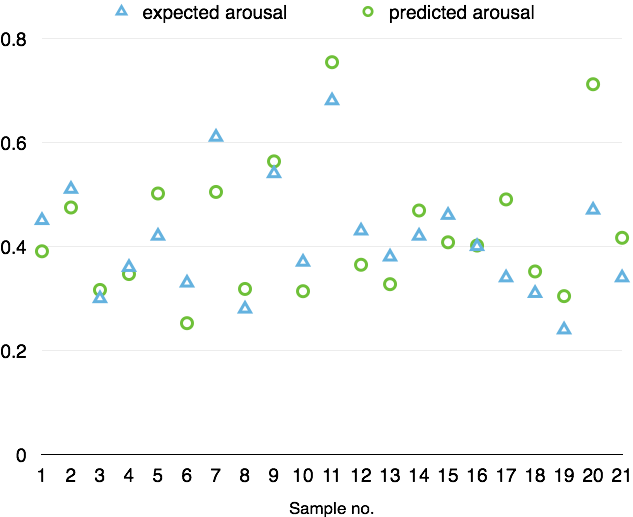
\includegraphics[width=0.7\textwidth]{Figures/finalarousal}
    \centering

  \caption{A plot of the expected and predicted .}
  \label{fig:anneval}
\end{figure}


We wanted to use neural networks to calculate valence and arousal ratings of songs using audio features we extract. 

We computed the mean error between participant ratings and network-predicted outputs across all segments of all test melodies. The network's performance total RMSE was 0.088954243616 on scale from 0 to 1. or 21.62\%.
The network predicted at an average accuracy of 78.38\% for all 20 segments. The plot of the expected and predicted values can be seen in Figure \ref{fig:anneval}.
These results are more promising than ones of Yang and Lin cite{mood}, where their R^2 scored 58.3\% for arousal and 28.1\% for valence.\textit{•}


\begin{figure}[t]
    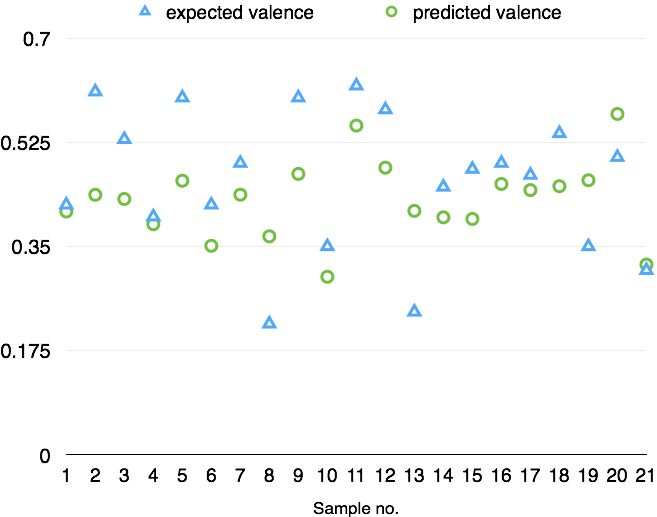
\includegraphics[width=0.7\textwidth]{Figures/finalvalence}
    \centering

  \caption{A plot of the expected and predicted .}
  \label{fig:anneval}
\end{figure}


Results from the static network indicate that a network can be trained to identify statistical consistencies across audio features abstracted from music and satisfactorily predict valence/arousal values that closely match mean participant ratings.


\begin{table}
\begin{center}
\begin{tabular}{| c | c | c | c | } \hline 
 expected arousal & expected valence & predicted arousal & predicted valence \\ \hline \hline

0.45  & 	0.42  &  0.390444 &  0.408524   \\ \hline
0.51	&  0.61  &  0.474538 & 0.436625   \\ \hline
0.3    &  0.53  &  0.316230 & 0.429643   \\ \hline
0.36	&  0.4    &  0.346713 & 0.387249   \\ \hline
0.42	&  0.6    &  0.501414 & 0.460295   \\ \hline
0.33	&  0.42  &  0.252398 & 0.350910  \\ \hline
0.61	&  0.49  &  0.504392 & 0.436785   \\ \hline
0.28	&  0.22  &  0.318096 & 0.366836   \\ \hline
0.54	&  0.6    &  0.563120 & 0.471717   \\ \hline
0.37	&  0.35  &  0.313782 & 0.298909   \\ \hline
0.68  &  0.62  &  0.753534 & 0.552922   \\ \hline
0.43	&  0.58  &  0.364568 & 0.482194   \\ \hline
0.38	&  0.24  &  0.327288 & 0.409628   \\ \hline
0.42  &  0.45  &  0.468762 & 0.398749   \\ \hline
0.46  &  0.48  &  0.407701 & 0.396029   \\ \hline
0.4    &  0.49  &  0.401469 & 0.454892   \\ \hline
0.34  &  0.47  &  0.490065 & 0.444592   \\ \hline
0.31  &  0.54  &  0.351714 & 0.451086   \\ \hline
0.24  &  0.35  &  0.304314 & 0.461078   \\ \hline
0.47	&  0.5    &  0.711224 & 0.572459   \\ \hline
0.34	&  0.31  &  0.416320 & 0.319491   \\ \hline


\end{tabular}
\caption{Table showing the root mean square error for training the network for given number of nodes in the hidden layer.}
\label{table:rsmetablefinal}
\end{center}
\end{table}


\subsection{Comparison to Original Songs}
In order to evaluate the quality of the gameplay generated by our program, we will test our game with songs already existing in the original Guitar Hero game and compare the output we get with its already defined levels. However, to make that possible, the music track we feed to our program must be an instrumental version of the same song as Guitar Hero's songs are mapped onto the key presses by looking at the guitar line of the song, not the main melody. We can then create statistics of correctly identified, false alarm and missed buttons.

\subsection{Melody Extraction Testing}
To evaluate our implementation of the melody extraction algorithms we can use the technique used at Music Information Evaluation eXchange, described in section 2.4.3 of the report. In particular, we can compare the performance of our implementation when tested on the samples used during MIREX to the official statistics presented in papers \cite{salamon, comparison}.

Another way of evaluating the game is creating a set of songs and generating levels for them. After that a trained Guitar Hero player can play those levels. If the buttons were consistently on time with the notes then the melody extraction and game synchronisation techniques are considered to work.

\subsection{Questionnaires}
Questionnaires are one of the most common and popular tools to gather data from a large number of people. They generally consist of a limited number of questions that ask participants to rate the effectiveness of various aspects of the activity. The questions should focus on the key points we are trying to evaluate. 

Questionnaires tend to be short in order to reduce the amount of time respondents need to complete them, and therefore increase the response rate. 

We plan on writing questions that are quantitative and generally consist of close-ended questions (tick the box, or scales), as the open ended questions tent to make data analysis and reporting more difficult.